\documentclass{beamer}

\providecommand{\rootdir}{../doc}

% \def\privateData{private_data}

% % % % % % % % % % % % % % % % % % % % % % % % % % % % % % % % % % % % % % % %

\usepackage[english]{babel}
\usepackage{ifthen}
\usepackage{color}
\usepackage{hhline}
\usepackage{adjustbox}
\usepackage{amsmath,amsfonts, amssymb}
\usepackage{mdframed}

\usepackage{tikz, skak}
\usetikzlibrary{fit, matrix, positioning, shapes, decorations.pathreplacing,
                shapes.geometric, chains, arrows, calc }




\newcommand{\red}[1]{{\color{red} #1}}
\newcommand{\green}[1]{{\color{green!50!black} #1}}
\newcommand{\orange}[1]{{\color{orange} #1}}
\newcommand{\blue}[1]{{\color{blue} #1}}


\newcommand{\resizeinput}[2][1]{%
  \resizebox{#1\textwidth}{!}{\input{#2}}%
}

% % % % % % % % % % % % % % % % % % % % % % % % % % % % % % % % % % % % % % % %
% from MathDefs.tex

\def\Re{\mathbb{R}}

\def\behaviour{\mathrm{behaviour}}
\def\act{\mathrm{act}}
\def\react{\mathrm{react}}
\def\state{\mathrm{state}}
\def\action{\mathrm{action}}
\def\msg{\mathrm{message}}

\def\coh{\mathrm{coh}}
\def\rel{\mathrm{rel}}
\def\fold{\mathit{fold}\,}

\def\Bool{\mathrm{Bool}}
\def\Candidate{\mathit{Candidate}}
\def\Details{\mathit{Details}}
% \def\Context{\mathit{Context}}


\providecommand{\letIn}[2]{
  \begin{aligned}[t]%
    & \mathit{let}\, #1 \\%
    & \mathit{in}~ #2%
  \end{aligned}%
}


% % % % % % % % % % % % % % % % % % % % % % % % % % % % % % % % % % % % % % % %

% https://tex.stackexchange.com/questions/45938/error-when-using-colour-in-author
\ifthenelse{\isundefined{\privateData}}
           {\author{\texorpdfstring{\color{red} Anonymous}{???}}}
           {\input{\privateData}}

% % % % % % % % % % % % % % % % % % % % % % % % % % % % % % % % % % % % % % % %

\title{University class schedule generation using personalizable agents negotiation}
\subtitle{Thesis for Master of Science in Intelligent Systems}
\institute[ITESM]{Tecnol\'{o}gico de Monterrey}
\logo{\includegraphics{../doc/escudo-itesm}}
\date{May, 2017}

% % % % % % % % % % % % % % % % % % % % % % % % % % % % % % % % % % % % % % % %


\mode<presentation>

\begin{document}

\frame{\titlepage}

% % % % % % % % % % % % % % % % % % % % % % % % % % % % % % % % % % % % % % % %
% % % % % % % % % % % % % % % % % % % % % % % % % % % % % % % % % % % % % % I
\section{University Class Scheduling Problem (UCSP)}
\subsection{The Problem}

\begin{frame}{University Class Scheduling Problem}
  \begin{block}{The Problem}
    \textbf{U}niversity \textbf{C}lass \textbf{S}cheduling \textbf{P}roblem (UCSP)
    consists in finding valid \alert{class} assignations for \underline{all} the
    participants:
    \begin{itemize}
      \item Groups / Students
      \item Professors
    \end{itemize}
  \end{block}
  \begin{block}{Class}
    A class is an educational event, that is formed with purpose of studying
    some \alert{discipline}.
    \begin{columns}
      \begin{column}{4cm}
        \\Takes place
        \begin{itemize}
          \item in a \underline{classroom}
          \item on given \underline{day}
          \item during given \underline{time}
        \end{itemize}
      \end{column}
      \begin{column}{3cm}
        Links together
        \begin{itemize}
          \item a \underline{group} and
          \item a \underline{professor}
        \end{itemize}
      \end{column}
    \end{columns}

  \end{block}
\end{frame}

\begin{frame}
  \begin{columns}
    \begin{column}{4cm}
      \begin{block}{Schedule}
        The complete schedule consists of all the classes of all the participants,
        that can be seen as points in 5-dimensional space. It can be decomposed
        into a set of \alert{timetables}.
      \end{block}
    \end{column}
    \begin{column}{7cm}
        \resizeinput{\rootdir/img/ScheduleHypercube/GRPT-content.tikz}
    \end{column}
  \end{columns}
\end{frame}

\begin{frame}
  \begin{block}{Timetable}
    Timetable is projection of the schedule on the person/entity.
    It is a 2-dimensional table, that contains \underline{only} the classes
    of projection target.
  \end{block}
  \begin{columns}
    \begin{column}{.5\textwidth}
      \centering
      \begin{tabular}{|c||c|c|c|}
  \hline & Mon & Tue & $\cdots$ \\
  \hhline{|=#=|=|=|}
  08:30 -- 08:40 & x & & \\\hline
  08:40 -- 08:50 & x & & \\\hline
  08:50 -- 09:00 & x & & \\\hline
  $\vdots$\quad~--~\quad$\vdots$ & & & \\\hline
  09:50 -- 10:00 & x & & \\\hline
  10:00 -- 10:10 &   & & \\\hline
  10:10 -- 10:20 & y & & \\\hline
  10:20 -- 10:30 & y & & \\\hline
  $\vdots$\quad~--~\quad$\vdots$ & & & \\\hline
\end{tabular}

    \end{column}
    \begin{column}{.5\textwidth}
      \centering
      \begin{tabular}{|c||c|c|c|}
  \hline & Mon & Tue & $\cdots$ \\
  \hhline{|=#=|=|=|}
  08:30 -- 09:15 & x & & \\\hline
  09:25 -- 10:10 & x & & \\\hline
  10:30 -- 11:15 & y & & \\\hline
  11:25 -- 12:10 & y & & \\\hline
  Lunch          &   & & \\\hline
  13:25 -- 14:10 & z & & \\\hline
  14:20 -- 15:05 & z & & \\\hline
  15:25 -- 16:10 &   & & \\\hline
  $\vdots$\quad~--~\quad$\vdots$ & & & \\\hline
\end{tabular}

    \end{column}
  \end{columns}
  % \centering
  % \begin{tabular}{|c||c|c|c|c|c|c|}
  \hline & Mon & Tue & Wed & Thu & Fri & Sat \\
  \hhline{|=#=|=|=|=|=|=|}
  08:00 -- 08:30 & x & & & w & & \\\hline
  08:30 -- 09:00 & x & & & w & & \\\hline
  09:00 -- 09:30 & x & & & z & & \\\hline
  09:30 -- 10:00 & y & & & z & & \\\hline
  10:00 -- 10:30 & y & & & z & & \\\hline
  $\vdots$\quad~--~\quad$\vdots$ & & & & & & \\\hline
  21:00 -- 21:30 &   & & & & & \\\hline
  21:30 -- 22:00 &   & & & & & \\\hline
\end{tabular}

\end{frame}

% % % % % % % % % % % % % % % % % % % %
\subsection{Constraints}

\begin{frame}[label=constraints]{University Class Scheduling Constraints}
  \fbox{
    \begin{columns}[t]
      ~~Independent
      \begin{column}{.4\textwidth}
        \begin{block}{Class}
          \begin{itemize}
            \item Group needs
            \item Professor can teach
            \item Classroom is suitable
          \end{itemize}
        \end{block}
      \end{column}
      \begin{column}{.4\textwidth}
        \begin{block}{Time}
          \begin{itemize}
            \item Classes non intersection
          \end{itemize}
        \end{block}
      \end{column}
    \end{columns}
  }
  \\[.7cm]
  \fbox{
    \begin{columns}[t]
      Personal
      \begin{column}{.4\textwidth}
        \begin{block}{Obligations}
          \begin{itemize}
            \item Personal \alert{strong} restrictions
          \end{itemize}
        \end{block}
      \end{column}
      \begin{column}{.4\textwidth}
        \begin{block}{Preferences}
          \begin{itemize}
            \item Personal \alert{weak} restrictions
          \end{itemize}
        \end{block}
      \end{column}
    \end{columns}
  }
\end{frame}

\input{Part-2}
\input{Part-3}
% % % % % % % % % % % % % % % % % % % % % % % % % % % % % % % % % % % % % % IV
\section{Coherence}

\begin{frame}
  \begin{block}{Coherence}
    In simple worlds, \emph{coherence} is a state or measure of some \emph{pieces}
    fitting together into a whole. Coherence can be applied to almost any aspect of
    the universe.
  \end{block}
  \begin{quote}
    The consistency or \emph{coherence} within a logical or mathematical
    system, means that $p$ and $\neg p$ must not be derivable from the
    basic assumptions in accordance with the observance of the syntactical
    rules (Daya, 1960).
  \end{quote}
  \begin{quote}
    Coherence theory is a psychologically motivated motivational cognitive theory with
    foundations in philosophy that approaches problems in terms of the satisfaction
    of multiple constraints within networks of highly interconnected elements
    (Sindhu, 2010).
  \end{quote}
\end{frame}


\begin{frame}{Coherence}
  \begin{block}{Coherence by Thagard}
    Thagard (1998) claimed that \alert{coherence} can be understood in terms of
    \alert{maximal satisfaction of multiple constraints}.

    \medskip
    By Thagard, coherence problem is about \underline{partitioning a graph} of
    \emph{information pieces}, interconnected by positive or negative weighted
    constraints, that enhance or diminish partition's coherence.
  \end{block}
\end{frame}
\begin{frame}{Coherence}
  \begin{block}{Information Graph Splitting}
    The information graph $\mathcal{V}$ consists of
    classes $C_1,\dots,C_4$, also there are three possibilities for
    class $C_1$ placement and two for class $C_4$.\\\bigskip
    \begin{columns}
      \begin{column}{.3\textwidth}
        \includegraphics[width=\textwidth, trim={20pt 20pt 100pt 20pt}]
                        {\rootdir/img/UAB-splitting.png}
      \end{column}
      \begin{column}{.8\textwidth}
        \qquad\quad A relation is
        \begin{mdframed}[leftmargin=2cm, hidealllines=true]
          \begin{itemize}
            \item[\red{\emph{inconsistent}}], if two classes intersect in time;
            \item[\orange{\emph{same class}}], if two classes differ only by time;
            \item[\green{\emph{consistent}}], otherwise.
          \end{itemize}
        \end{mdframed}
      \end{column}
    \end{columns}
  \end{block}
\end{frame}

% % % % % % % % % % % % % % % % % % % %
\subsection{Contexts}

\begin{frame}{Coherence}
  \begin{block}{Contexts}
    Describe aspects of coherence problem.
    \begin{columns}[t]
      \begin{column}{.5\textwidth}
        \begin{block}{Original}
          Proposed by Sindhu (2010) \\\medskip
          \begin{itemize}
            \item Contexts represent BDI
            \item Each context has own logic
            \item Contexts are connected by
                  \emph{bridge rules}
          \end{itemize}
        \end{block}
      \end{column}
      \begin{column}{.5\textwidth}
        \begin{block}{Proposed}
          \begin{itemize}
            \item Contexts represent groups of constraints
            \item \underline{Assess coherence}
                  of the given information and tell whether
                  it is \underline{coherent}
            \item Candidate is \alert{\underline{propagated}} through
                  the contexts
          \end{itemize}
        \end{block}
      \end{column}
    \end{columns}
  \end{block}
\end{frame}

\againframe{constraints}

\begin{frame}{Contexts}
  \begin{columns}
    \begin{column}{.2\textwidth}\end{column}
    \begin{column}{.2\textwidth}
      \tikz\draw[->, >=stealth, double, thick]
                (0,0)  node[yshift=10pt] {Candidate $\tilde{c}$}
                  --
                (0,-5) node[yshift=-10pt] {Assessed candidate $\tilde{c}$};
    \end{column}
    \begin{column}{.5\textwidth}
      \vfill
      \begin{enumerate}
        \item Common / Independent
          \begin{enumerate}
            \item Class constraints
            \item Time constraints
          \end{enumerate}
        \item Internal / Personal
          \begin{enumerate}
            \item Obligations (strong)
            \item Preferences (weak)
          \end{enumerate}
        \item \underline{External}\\
              communicates, works towards
              \emph{common goal}
      \end{enumerate}
      \vfill
    \end{column}
    \begin{column}{.3\textwidth}\end{column}
  \end{columns}
\end{frame}

% % % % % % % % % % % % % % % % % % % % % % % % % % % % % % % % % % % % % % V
\section{Agents}

\begin{frame}{Agents}
  The notion of agent appears in Aristotle's works
   \begin{quote}
     Entity that acts with a purpose, within a social context.
   \end{quote}\\\medskip
  The prætorian roman law defined an agent as
    \begin{quote}
      A person who acts on behalf of a principal for
      a specific purpose and under limited delegation of authority and
      responsibility.
    \end{quote}\\\medskip
  The earliest use of the term agent in AI was
    \begin{quote}
      A program that is capable of executing an action vicariously.
    \end{quote}
\end{frame}

% ?? Solve CSPs with Agents ??

\begin{frame}
  \centering
  \begin{block}{An Agent}
    is \emph{computer system}, that
    \begin{enumerate}
      \item has a degree of autonomy in determining its behavior,
      \item interacts with humans and or other agents,
      \item perceives the environment and reacts to it, and
      \item exhibits a goal directed behavior.
    \end{enumerate}
  \end{block}
  \begin{block}{A Negotiation}
     is a process of \underline{communication} between heterogeneous agents
     with goal of resolving some common problem.
  \end{block}
  \begin{block}{A Negotiating Agent}
     is an \emph{isolated} \emph{proactive} computational entity,
     capable of sending and receiving messages.
  \end{block}
\end{frame}

\begin{frame}{Agents}
  \begin{block}{Behaviour}
    An agent is defined by it's behaviour:
    \begin{align*}
      \behaviour_\act   &: \state \mapsto \action \\
      \behaviour_\react &: \state \times \msg \mapsto \action
    \end{align*}
    % The agents must use a common \emph{communication protocol}, to ensure
    % understanding between agents of the same or different roles.
  \end{block}
  \begin{block}{Role}
    A role describes whom or what an agents represents in the negotiation and
    defines \emph{behaviour archetype}.
  \end{block}
  \begin{block}{Implementation}
    Agents are implemented in \underline{Haskell} using
    \emph{Software Transactional Memory} (STM)
    --- a promising concurrency paradigm.
  \end{block}
\end{frame}

% % % % % % % % % % % % % % % % % % % % % % % % % % % % % % % % % % % % % % % %




% % % % % % % % % % % % % % % % % % % % % % % % % % % % % % % % % % % % % % VI
\section{Agent Roles}

\begin{frame}{Agent Roles}

  \begin{center}
  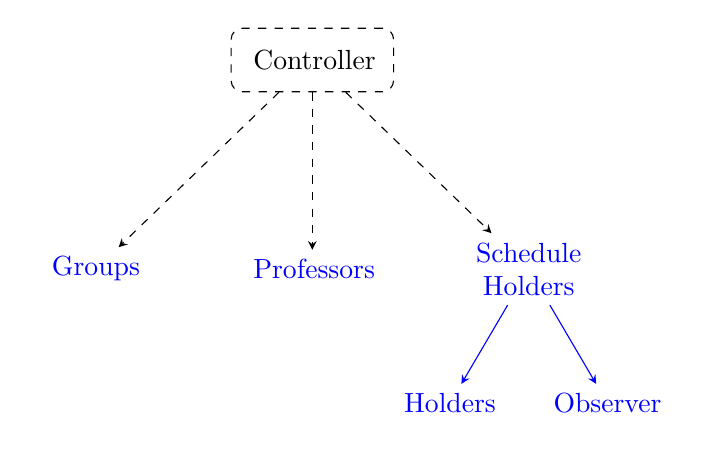
\begin{tikzpicture}[every node/.style={text width=1.5cm, align=center}]
    \node[draw, rounded corners,dashed, inner sep=8pt] (C) {Controller};
    \node[color=blue, below=2cm of C] (P) {Professors};
    \node[color=blue, left=of P]  (G) {Groups};
    \node[color=blue, right=of P] (H) {Schedule Holders};
    \draw[->, >=stealth, dashed] (C) -- (G);
    \draw[->, >=stealth, dashed] (C) -- (P);
    \draw[->, >=stealth, dashed] (C) -- (H);
    \node[color=blue, below=of H, xshift=-1cm] (HH) {Holders};
    \node[color=blue, below=of H, xshift=1cm]  (HO) {Observer};
    \draw[->, >=stealth, blue] (H) -- (HH);
    \draw[->, >=stealth, blue] (H) -- (HO);
  \end{tikzpicture}
  \end{center}

  \bigskip

  \blue{Groups} and \blue{Observer} have \underline{active} behaviour, while \\
  \blue{Professors} and \blue{Holders} exhibit only the \underline{reactive} one.

\end{frame}

% % % % % % % % % % % % % % % % % % % %
\subsection{Group}


% % % % % % % % % % % % % % % % % % % % Candidates Creation

\againframe{candidate-def}

\begin{frame}{Group: Candidates Creation}
  \centering
  Each class consists of \emph{class-core} and \emph{instance} assignations

  \bigskip \bigskip

  \begin{block}{Class-Cores Pool}
    is a lazy random sequence of class-cores,
    that contain \underline{a class for each discipline}, needed by the group.

    \medskip

    \begin{enumerate}
      \item For each discipline needed select professors, that can teach it.
            Randomize professors lists.
      \item Lazily generate all possible combinations \emph{professor} -- \emph{discipline}.
      \item When getting next combination, assign the generating \emph{group}.
    \end{enumerate}
  \end{block}
\end{frame}

\begin{frame}{Group: Candidates Creation}
  \begin{block}{Day -- Time -- Room}
    \begin{enumerate}
      \item Generate random \emph{day}.
      \item Select random \emph{classroom}.
      \item Generate \emph{beginning time}.
      \item Get class duration from the \emph{discipline}, contained in argument class-core.
            Calculate \emph{end time}.
      \item Test \emph{end time} consistency (upper bound).
      \item Test \emph{time consistency} of the values from (1-4) using the history.
      \item If new values are consistent, add them to history, assign to class-core
            and return it.
            Otherwise, repeat from (1).
    \end{enumerate}
    Assignation for classes of same possible candidate is done with same
      history.
  \end{block}
\end{frame}


% % % % % % % % % % % % % % % % % % % % Action

\begin{frame}{Group Action}
  \marginbox{-30pt 0 0 0}{
    \clipbox{-65pt 350 20 0}{ %{left bottom right top}
      \resizebox{\textwidth}{!}{
        \input{\rootdir/img/SolutionProcess-content.tikz}
      }
    }
  }
\end{frame}

% \subsubsection{Candidate Modification}
% \subsubsection{Sleep and Awake, Solution Improvement}


% % % % % % % % % % % % % % % % % % % %
\subsection{Professor}
\subsubsection{Reactive}
\subsubsection{Solution Improvement}

% % % % % % % % % % % % % % % % % % % %
\subsection{Schedule Holders}
\subsubsection{Putting Candidates Together}
\subsubsection{Conflicts and Forced Resolution}
\subsubsection{Schedule Observation}

% % % % % % % % % % % % % % % % % % % %
\subsection{Common / Conflicts Resolution}
\subsubsection{Deep Coherence Assessment}
\subsubsection{Candidate ``Rareness''}

% % % % % % % % % % % % % % % % % % % % % % % % % % % % % % % % % % % % % % VII
\section{Improvements}
\subsection{Students Representation}
\subsection{Classrooms Representation}
\subsection{Roles Extension}

% % % % % % % % % % % % % % % % % % % % % % % % % % % % % % % % % % % % % % VIII
\section{Results}
%% ??? TODO ???



\end{document}
